\subsection{Framework Architecture}
\label{sec:architecture}

The framework separates \emph{what} is modeled from \emph{how} a specific city supplies it. A common computational core defines the territorial model, the routing procedure, and the indicator set, while everything that varies across municipalities — data paths, penalty parameters, and scenario composition — is declared in configuration. The core is organized into modules with distinct responsibilities: \texttt{grid} and \texttt{network} build the spatial support, \texttt{pois} and \texttt{environment} load destinations and environmental layers, \texttt{penalties} rewrites edge costs, \texttt{routing} computes distance matrices, and \texttt{demographics} and \texttt{indicators} produce the socioeconomic and accessibility measures. A new city requires no change to these modules, only a new configuration file, and the comparison between a typical and a conditioned scenario follows from the same implementation.

Figure~\ref{fig:framework} summarizes the flow. The left panel shows the network under the typical scenario, with its original travel costs. The central panel shows the penalization mechanism, which uses environmental data to rewrite the cost of the mobility infrastructure. The right panel shows the conditioned scenario, where longer edges represent the added time or cost caused by the disruption.

\begin{figure}[H]
  \centering
  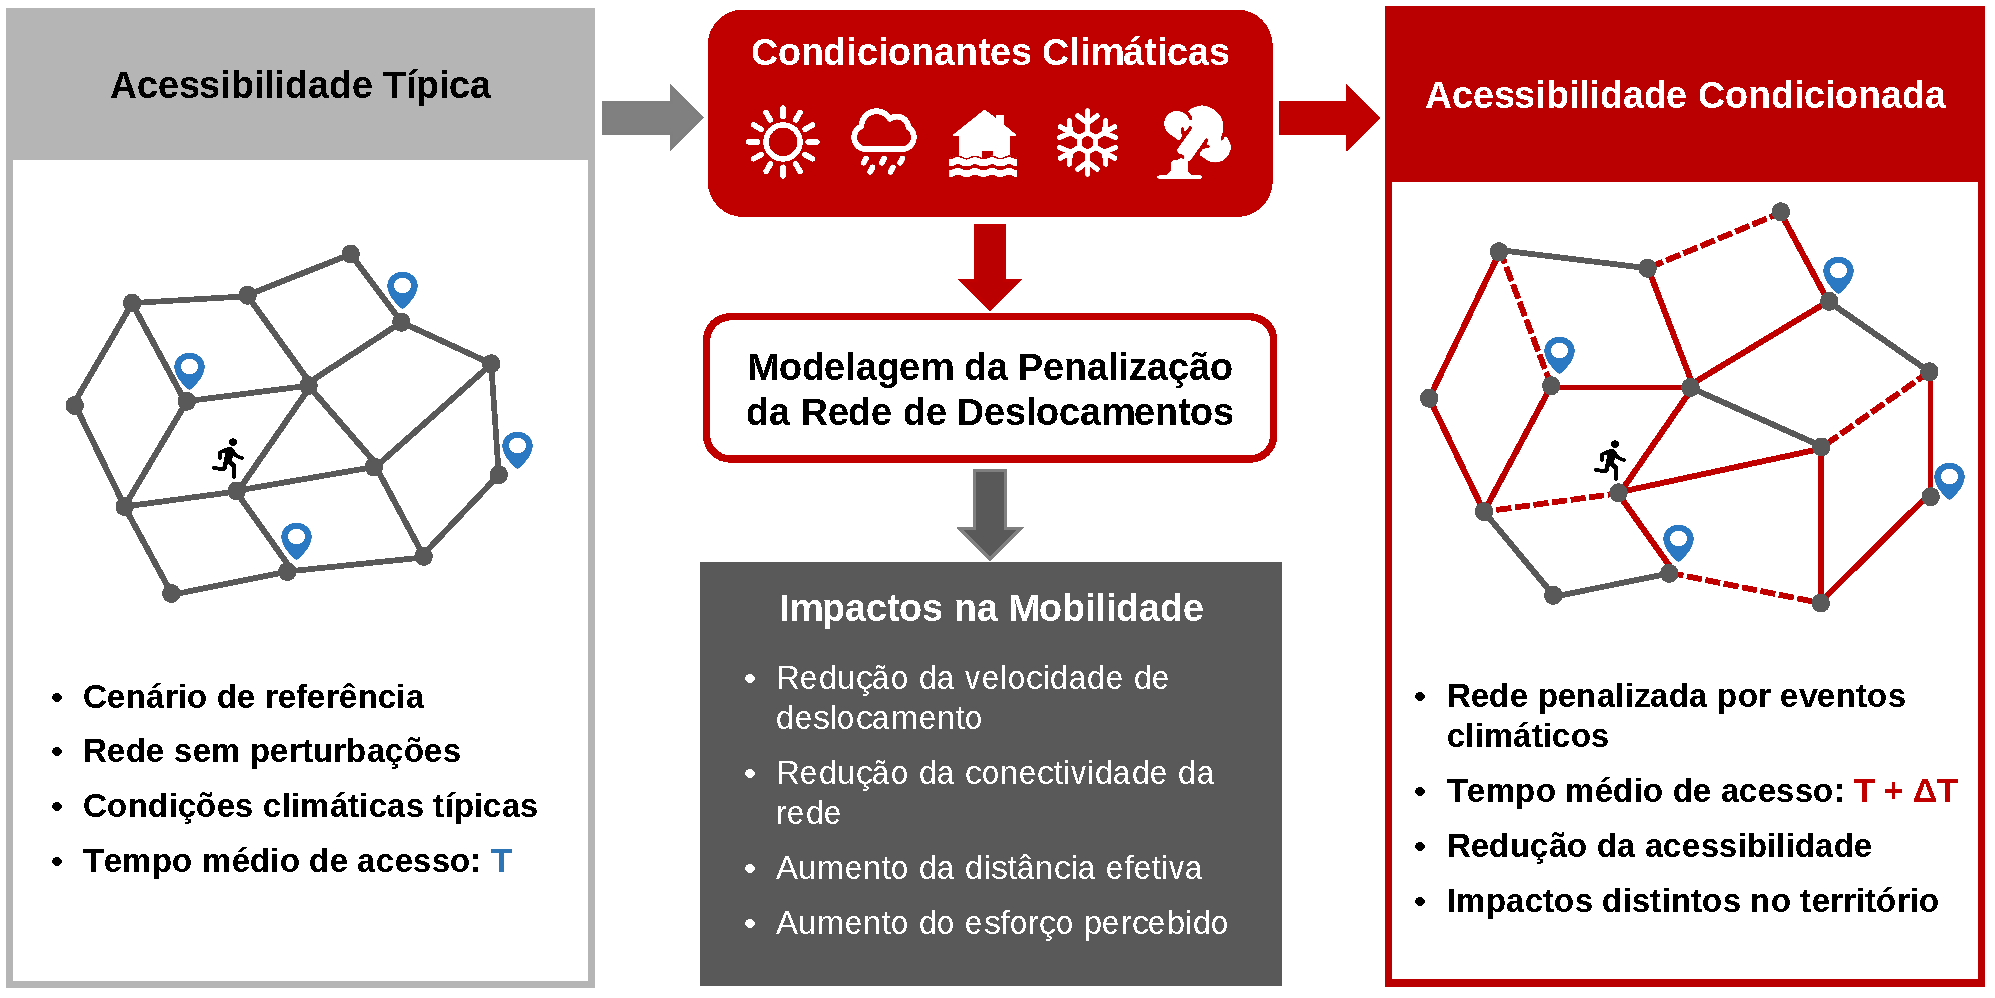
\includegraphics[width=1\textwidth]{figs/framework.pdf}
  \caption{Modeling flow for accessibility scenarios. Edges lengthen as their travel cost increases, so the geometry in the right panel encodes the effect of the disruption rather than the physical street layout.}
  \label{fig:framework}
\end{figure}

\subsubsection{Territorial Modeling}
\label{subsec:territorial_modelling}

The urban territory is assembled from four data types that differ in geometry, resolution, and coordinate reference system, and whose integration is the first source of complexity in the pipeline.

\begin{description}
  \item[Analysis grid.] A regular partition of the territory defining the minimum unit of study. The library supports hexagonal and square cells; the side or radius is a parameter set according to the transport mode and the local context. With hexagonal cells, the distance between neighboring centroids is uniform in all six directions, which avoids the directional bias that square cells introduce in neighborhood-based aggregation. The centroid of each cell is the theoretical origin of trips and the basis for computing and aggregating indicators.
  \item[Points of interest (POIs).] The destinations of trips: coordinates locating the everyday services used by the population, organized into categories such as health, education, and transport. Their selection depends on the availability of local databases, whether official or crowdsourced. Each POI is snapped to the nearest network vertex before routing, so the reachable set is bounded by the network rather than by straight-line distance.
  \item[Street network.] The mobility infrastructure is structured as a spatial graph, with vertices at intersections and edges along street segments whose initial base weight is travel time. Each cell centroid is attached to the nearest network vertex, and a maximum snap distance discards cells whose centroid lies too far from the network — a parameter that prevents a cell in an unmapped area from being routed through a vertex several kilometers away. Because this threshold removes cells from the analysis, it must be reported alongside the results.
  \item[Environmental layers.] Spatial layers that may be continuous, such as raster images, or discrete, such as vector polygons, mapping the climate or environmental phenomena under evaluation. A single scenario may stack several such layers. They are overlaid on the street network to adjust the travel cost of affected edges, as described in Section~\ref{sec:penalization}.
\end{description}

A fifth input completes the model. \textbf{Demographic and socioeconomic data} characterize the resident population — density, income, and schooling — and come from official censuses. These data are published in irregular administrative units such as census tracts, which do not align with the analysis grid, so each tract attribute is transferred to the cells by area-weighted mean: a cell receives the average of the tract values covering it, weighted by the intersected area. Where a tract has no value, its area is excluded from the denominator, so a cell partially covered by suppressed data is not diluted toward zero. The numerator and denominator are both taken from tracts with data, which keeps the cell value equal to the value of its contributing tracts rather than to a fraction of it.

This distinction between interpolation by density and aggregation by area is not interchangeable. Density interpolation conserves totals and suits population counts; area-weighted averaging preserves the value of the attribute itself and suits rates and indices. Population is interpolated the first way, socioeconomic indices the second.
